\section{Finding Clusters} \label{sect:finding}


\begin{figure}
    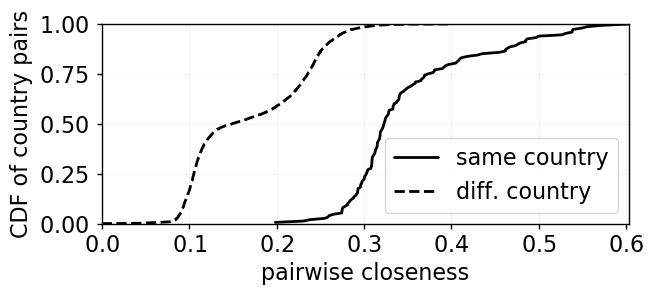
\epsfig{file=figs/country_cdf.png}
    \caption{Dendrogram}
\end{figure}


\begin{figure}
    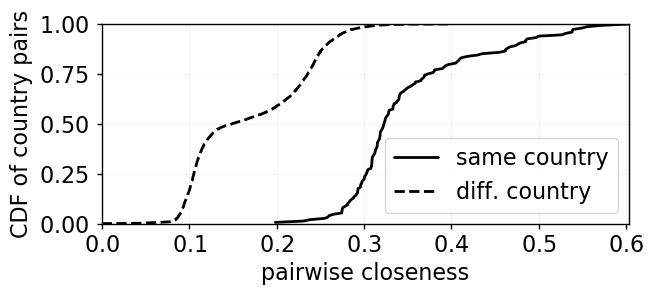
\epsfig{file=figs/country_cdf.png}
    \caption{CRNE distance vs geo-distance (is this redundant?)}
\end{figure}


\begin{figure}
    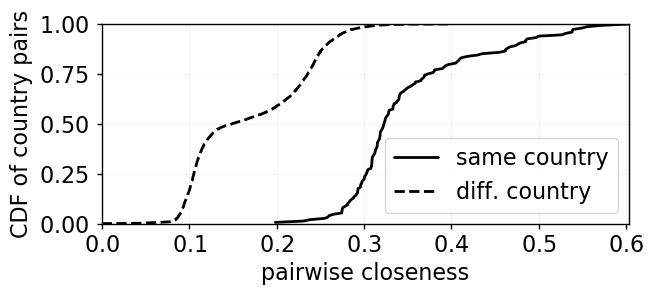
\epsfig{file=figs/country_cdf.png}
    \caption{CRNE distance vs bit distance (does this make sense?)}
\end{figure}

\begin{figure}
    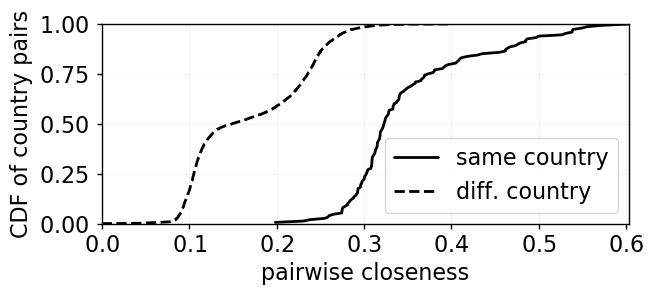
\epsfig{file=figs/country_cdf.png}
    \caption{CRNE distance vs median-latency ratio (does this make sense?)}
\end{figure}


\begin{figure}
    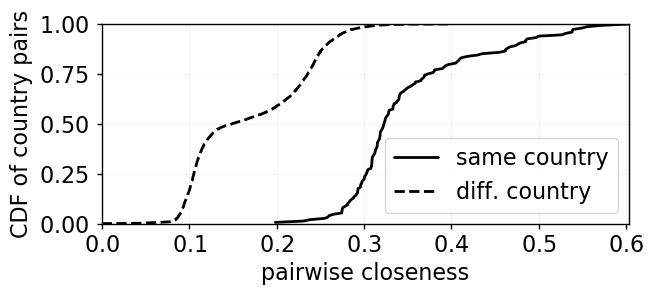
\epsfig{file=figs/country_cdf.png}
    \caption{Completeness / homogeneity for [country / ASN / bgp prefix / 24 / local resolver] vs clustering distance threshold (this will either be several lines on one plot or an array of subplots)}
\end{figure}
